\documentclass[11pt]{article}

\usepackage[T1]{fontenc}
\usepackage{lmodern}
\usepackage[margin=1.0in]{geometry}
\usepackage{amsmath,amssymb,amsthm,mathtools}
\usepackage{microtype}
\usepackage{graphicx}
\usepackage[hidelinks]{hyperref}
\usepackage{enumitem}

\setlist{nosep}
\newtheorem{theorem}{Theorem}
\newtheorem{proposition}{Proposition}
\theoremstyle{remark}
\newtheorem{remark}{Remark}

\newcommand{\T}{\mathbb T}
\newcommand{\C}{\mathbb C}
\newcommand{\B}{\mathcal B}
\newcommand{\Hh}{\mathcal H}
\newcommand{\Ee}{\mathcal E}
\newcommand{\ran}{\operatorname{ran}}
\newcommand{\rank}{\operatorname{rank}}

\title{Necessity of the Analytic--Injective Criterion\\for Finite-Rank Spectral Densities}
\author{Independent research note}
\date{August 17, 2026}

\begin{document}
\maketitle

\begin{abstract}
Dritschel--Rovnyak ask whether their analytic--injective multiplier
criterion for factorability is necessary, recording only dimensions one and
two as known.  We prove necessity whenever the outer spectral factor has
finite-dimensional output.  This settles every finite-dimensional Hilbert
space and, more generally, every factorable operator-valued function of
uniformly finite rank on an arbitrary separable Hilbert space.  The proof
factors the finite-dimensional co-Gramian and then uses equality of Gram
operators to construct a measurable partial isometry.  We also isolate the
precise analytic-minorant problem left in infinite dimension.
\end{abstract}

\section*{Packet status}

\begin{description}[leftmargin=3.0cm,style=nextline]
\item[Run] \texttt{fa\_banach\_001}, lane 13.
\item[Source] arXiv:0903.3639, Theorem~4.3 and the question on PDF page~14 \cite{DR}.
\item[Classification] Candidate strong partial result, likely valid subject to human review.
\item[Novelty] Moderate.  No later explicit answer or all-finite-dimensional extension was located.
\end{description}

\begin{center}

\includegraphics[width=0.96\textwidth]{figures/source_question.png}
\end{center}

\section{Statement}

Let $F\in L^\infty_{\B(\Hh)}(\T)$ be positive.  Following the source,
$F$ is \emph{factorable} if
\[
 F(\zeta)=A(\zeta)^*A(\zeta)\quad\text{a.e.}
\]
for an operator-valued Smirnov function $A$; the factor may be chosen outer.
Because $F$ is bounded, such an $A$ belongs to $H^\infty_{\B(\Hh)}$.

\begin{theorem}[finite-output necessity]\label{thm:main}
Suppose $F=A^*A$ with $A$ outer and
\[
 \overline{A H^2_{\Hh}}=H^2_{\Ee}
\]
for a finite-dimensional subspace $\Ee\subseteq\Hh$.  Then there is a
weakly measurable $\psi\in L^\infty_{\B(\Hh)}$ with
\begin{enumerate}[label=\textup{(\roman*)}]
\item $\psi F\in H^\infty_{\B(\Hh)}$;
\item $\psi(\zeta)$ is one-to-one on
$\overline{F(\zeta)\Hh}$ for almost every $\zeta$.
\end{enumerate}
Moreover $\|\psi\|_\infty\le1$, and $\psi(\zeta)$ is isometric on
$\overline{F(\zeta)\Hh}$ almost everywhere.
\end{theorem}

\begin{theorem}[two consequences]\label{thm:consequences}
The conditions in Theorem~4.3 of the source are necessary for factorability
in each of the following cases:
\begin{enumerate}[label=\textup{(\alph*)}]
\item $\dim\Hh<\infty$;
\item $\Hh$ is arbitrary and $\rank F(\zeta)\le r<\infty$ almost everywhere.
\end{enumerate}
Thus the dimensions one and two recorded in the source extend to every
finite dimension.
\end{theorem}

For reference, the source's sufficient criterion is reproduced below.
\begin{center}
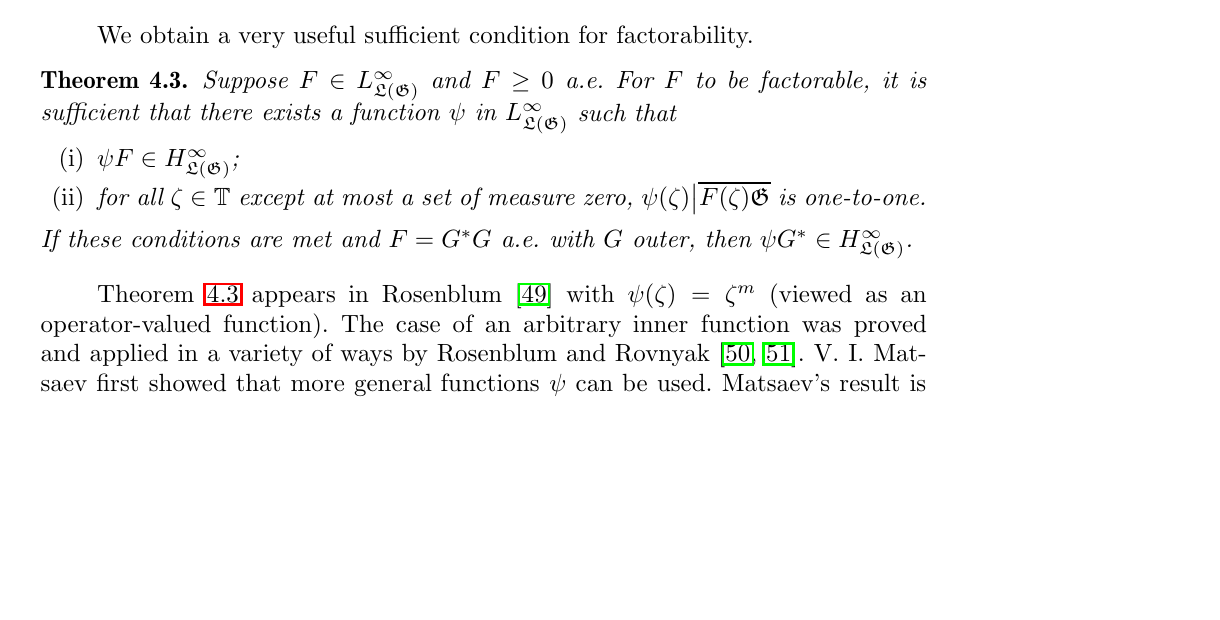
\includegraphics[width=0.94\textwidth]{figures/theorem_4_3.png}
\end{center}

\section{\hspace{0.18em}Factoring the co-Gramian}

We first separate the operator-theoretic step from the determinant argument.

\begin{proposition}[co-Gramian principle]\label{prop:cogram}
Let $F=A^*A$ with $A\in H^\infty_{\B(\Hh)}$.  Suppose, on a fixed closed
subspace $\Ee$ containing the ranges of $A$, that
\[
 AA^*=Q^*Q\quad\text{a.e.}
\]
for $Q\in H^\infty_{\B(\Ee)}$.  Then the conclusion of
Theorem~\ref{thm:main} holds.
\end{proposition}

\begin{proof}
At almost every boundary point the maps
\[
 A^*:\Ee\longrightarrow\Hh,
 \qquad Q:\Ee\longrightarrow\Ee
\]
have the same Gram operator:
\[
 (A^*)^*A^*=AA^*=Q^*Q.
\]
Therefore the rule $U(A^*y)=Qy$ defines an isometry from $\ran A^*$ to
$\ran Q$.  Extend it continuously to $\overline{\ran A^*}$ and by zero on
its orthogonal complement.  This gives a partial isometry
$U:\Hh\to\Ee$ satisfying $UA^*=Q$.  The standard measurable polar
decomposition makes $U(\zeta)$ weakly measurable; in finite dimensions it
is equivalently obtained using the measurable Moore--Penrose inverse.

Let $J:\Ee\hookrightarrow\Hh$ be the inclusion and put $\psi=JU$.  Then
$\|\psi\|\le1$, it is isometric on $\overline{\ran A^*}$, and
\[
 \psi F=JUA^*A=JQA\in H^\infty_{\B(\Hh)}.
\]
Finally
$\overline{\ran F}=\overline{\ran A^*}$ because the two spaces have the
same orthogonal complement $\ker A$.  This proves both required conditions.
\end{proof}

Now assume $r=\dim\Ee>0$ in Theorem~\ref{thm:main}.  Outerness implies
\begin{equation}\label{eq:zero-range}
 \overline{\ran A(0)}=\Ee.
\end{equation}
Indeed, approximate any constant function $e\in H^2_\Ee$ by functions
$Af_n$ and apply the bounded evaluation map at zero.  Since $\Ee$ is finite
dimensional, $A(0)$ is onto.

Choose an isometry $V:\C^r\to\Hh$ such that
$B(0):=A(0)V:\C^r\to\Ee$ is invertible, and set
\[
 W=AA^*,\qquad B=AV,\qquad \Delta=\det B.
\]
The scalar function $\Delta\in H^\infty$ is nonzero.  Since $VV^*\le I$,
\begin{equation}\label{eq:det-bound}
 W=AA^*\ge AVV^*A^*=BB^*,
 \qquad \det W\ge |\Delta|^2\quad\text{a.e.}
\end{equation}
Here determinant monotonicity is applied to positive $r\times r$ matrices.
The boundary values of a nonzero bounded analytic scalar function are
nonzero almost everywhere and $\log|\Delta|\in L^1(\T)$ after separating
positive and negative parts (Jensen's theorem).  Inequality~\eqref{eq:det-bound}, together
with the boundedness of $W$, yields
\[
 \log\det W\in L^1(\T),
 \qquad W(\zeta)>0\quad\text{a.e.}
\]
The matrix Szeg\H{o} theorem quoted as Theorem~4.7 in the source now gives
$Q\in H^\infty_{\B(\Ee)}$ such that $W=Q^*Q$.  (Boundedness follows from
$\|Q\|^2=\|W\|$ on the boundary.)  Proposition~\ref{prop:cogram} proves
Theorem~\ref{thm:main}.

\begin{center}
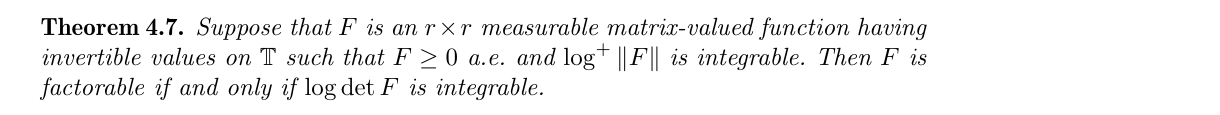
\includegraphics[width=0.94\textwidth]{figures/matrix_szego_theorem.png}
\end{center}

\section{\hspace{0.18em}Finite rank and the remaining problem}

Case (a) of Theorem~\ref{thm:consequences} is immediate from
Theorem~\ref{thm:main}.  For (b), boundary rank satisfies
$\rank A(\zeta)=\rank A(\zeta)^*A(\zeta)\le r$ almost everywhere.  Given
any $r+1$ domain vectors and $r+1$ output vectors, the corresponding scalar
minor of $A(z)$ is bounded analytic and has zero boundary values almost
everywhere; it therefore vanishes identically.  Hence
$\rank A(z)\le r$ throughout the disk.  Equation~\eqref{eq:zero-range}
then gives $\dim\Ee\le r$, so Theorem~\ref{thm:main} applies.

The argument also gives an exact gateway for the unsolved case.  Necessity
is equivalent to the existence of an analytic $K$ such that, almost
everywhere,
\begin{equation}\label{eq:minorant}
 K^*K\le CAA^*,\qquad \ker K=\ker A^*.
\end{equation}
Indeed, Douglas' lemma turns \eqref{eq:minorant} into $K=\psi A^*$; the
kernel identity supplies injectivity, and $\psi F=KA$ is analytic.  The
finite-dimensional determinant constructs $K=Q$.  In infinite dimension,
$AA^*+\varepsilon I$ regularization, compact smoothing, finite
compressions, weighted direct sums, and iteration of the source's Sarason
factorization were all audited.  Each loses the kernel equality or leaves
uncontrolled off-diagonal tails.  Conversely, a nonfactorable $AA^*$ is not
yet a counterexample, since \eqref{eq:minorant} need not dominate $AA^*$
from below.

A bounded literature search on August 17, 2026 covered the exact question,
later citations, and the phrases ``necessary for factorability'',
``$\psi F$'', ``$\psi G^*$'', and finite-dimensional spectral
factorization.  It found no later explicit answer or statement of the
extension above.  The result should therefore be read as a candidate new
partial answer, not as a claim that the unrestricted question is settled.

\begin{thebibliography}{9}
\bibitem{DR}
M.~A. Dritschel and J.~Rovnyak,
\emph{The Operator Fej\'er--Riesz Theorem}, arXiv:0903.3639 (2009).
\end{thebibliography}

\end{document}
